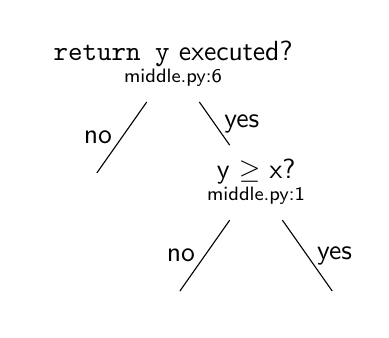
\begin{tikzpicture}[font=\sffamily, sibling distance=6em]
    \node {\begin{tabular}{c}\texttt{return y} executed? \\[-.4em] \scriptsize middle.py:6\end{tabular}}
	child {
        node {\PASS{}}
        edge from parent node[left]{no}
    }
	child {
        node {\begin{tabular}{c}y $\ge$ x? \\[-.4em] \scriptsize middle.py:1\end{tabular}}
        child {
            node {\FAIL{}}
            edge from parent node[left]{no}
        }
        child {
            node {\PASS{}}
            edge from parent node[right]{yes}
        }
        edge from parent node[right]{yes}
    };
\end{tikzpicture}